\section{Introducción}
\label{s1:sec:Introduccion}

\subsection{El juego}
\label{s1:subsec:elJuego}
El videojuego \pong es uno de los videojuegos más conocidos por todos,
publicado por Atari en 1972. \pong consiste en un juego para dos personas,
en el que el objetivo es hacer rebotar a una pelota para que el oponente no
pueda golpearla y pierda.
\begin{figure}[h]
  \centering
  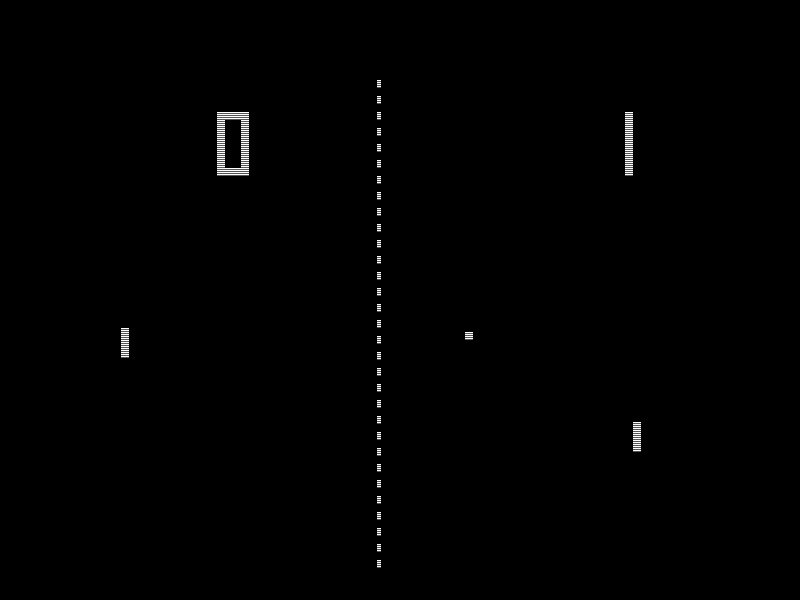
\includegraphics[width=0.4\textwidth]{images/pong.png}
  \caption{Imagen del juego original.}
  \label{s1:fig:pong}
\end{figure}

Para controlar la pelota, cada jugador dispone de una raqueta situada en
uno de los extremos de la pantalla, la cual únicamente pude desplazarse en
vertical. Cuando la pelota golpea una de estas raquetas, ésta cambia el
sentido horizontal de movimiento, dirigiéndose al otro jugador. Según en
que parte de la raqueta golpee la bola, ésta también modifica su componente
de movimiento vertical. De igual manera, cuando la pelota golpea el borde
superior o inferior del juego, también ve modificado su movimiento.  Se
considera que un jugador pierde cuando no es capaz de golpear la pelota y
ésta sale del juego por su lado de la pantalla.


\subsection{Descripción del proyecto}
\label{s1:subsec:objetivos}
El trabajo realizado consiste en el diseño e implementación del juego \pong
sobre una arquitectura distribuida formada por una FPGA Spartan~3~\cite{Spartan3}, y
dos maletines ARM S3C44B0X~\cite{maletinARM}, comunicados entre ellos
mediante UARTs.

La FPGA es el componente encargado de la lógica del juego. En él se
realizan todos los cálculos de posiciones y choques de la pelota. También
se lleva control de las puntuaciones. Además, sobre la FPGA se han
implementado dos módulos adicionales, uno encargado de la comunicación con
los maletines mediante UARTs, y otro para mostrar el juego en un monitor
VGA.\\
Los maletines ARM son utilizados para leer los movimientos de los jugadores
(mediante \rev{pulsadores y teclado matricial}) y comunicárselo a la FPGA
mediante una UART. Además, por motivos de diseño de la FPGA (sólo posee un
puerto UART), los maletines están diseñados para ser conectados en serie y
retransmitir los mensajes de un maletín al siguiente, hasta llegar a la
FPGA. La puntuación del juego también es mostrada por los \textit{display}
8-segmentos de la placa.

En la figura figura~\ref{s1:fig:vista_general_sistema} se puede ver una
descripción general del sistema.\\

\begin{figure}[h]
  \centering
  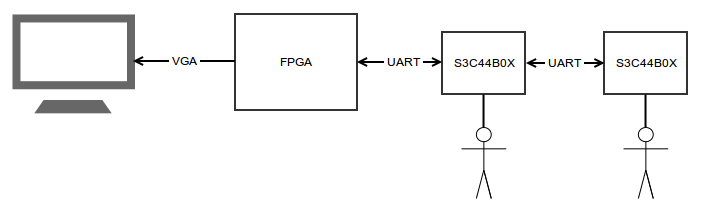
\includegraphics[width=0.8\textwidth]{images/descripcion_general.png}
  \caption{Descripción general del sistema.}
  \label{s1:fig:vista_general_sistema}
\end{figure}


La memoria está organizada de la siguiente forma:
en la sección~\ref{s2:sec:Disenyo} se muestra el modelado realizado por el
sistema, y diversos diagramas que describen el comportamiento del mismo. La
sección~\ref{s3:sec:Implementacion} muestra los aspectos más relevantes en
la implementación. Y para finalizar, la sección~\ref{s4:sec:Conclusiones}
muestra unas conclusiones y trabajo futuro a realizar si se desea seguir
con el proyecto.








%
%
%%%
%%% Local Variables:
%%% mode: latex
%%% TeX-master: "../main.tex"
%%% End:


